%
\section{Scenting technologies}
\label{sec:scenting-techn}
A scenting technology transforms an aromatic liquid into a gaseous fluid that
can be conveyed through the air and be captured by human olfactory sense,
usually for therapeutic or marketing purposes. As aforementioned in
Section~\ref{sec:context-motivation}, olfactory sense is the fastest way to the brain, thus, providing an exceptional
opportunity for marketing~\cite{news-harvard} --- ``75\% of the emotions we generate on a daily basis are affected by smell. Next
to sight, it is the most important sense we have''~\cite{lindstrom2006brand}.

In this section a brief overview of the scenting technologies is provided, with
special focus on ultrasonic diffusion as simple to control and cost-effective
solution.

\subsection{Overview}
\label{sec:overview}
There are several scenting technologies, mainly divided into~\cite{wen2019development}:
\begin{item-c}
\item \emph{Atomization}: it dispense odorants by transforming them into a
  gaseous fluid without requiring to heat. Its advantages are
  the dispensing process is fast and the dispensing quantity is controllable.
\item \emph{Thermalization}: it dispense odorants by vaporizing odor sources in
  the liquid state of the solid state using \gls{pwm} heaters. It requires a
  temperature controller to avoid scorching odor sources.
\item \emph{Evaporation}: it dispense odorants by conveying the liquid through a
  porous material into the outer surface (capillary action) where it evaporates
  naturally. It is a passive method, thus, not controllable.
\end{item-c}

The thermalization process requires heat which can modify fragrances, besides
requiring more power. Evaporation is a passive method, hence, not
controllable. Thus, one will focus on the \textbf{atomization} processes.

There are several atomization processes, with the most commercially relevant being~\cite{aromaUltrasonicVsNebul}:
\begin{item-c}
\item \emph{Ultrasonic diffusers}: it contains reservoirs for water and
  essential aromatic oils. It uses mechanical ultrasonic vibrations to
  brake down water molecules into droplets, producing mist, diffusing the oils
  into the air. Its advantages are: low power consumption, easy to clean,
  silent operation, and
  they double as a humidifier (can be a disadvantage too). Furthermore, they are
  a very cost-effective solution: the units themselves tend to cost less than
  nebulizing diffusers on average, but more importantly, ultrasonic diffusers
  use much less oil than nebulizing diffusers. They also run for longer periods
  of time, in several cases up to 24 hours before needing to be refilled.
  As a disadvantage they change the fragrance composition by incorporating water
  into it (this is not critical).
\item \emph{Nebulizers}:
  Nebulizing diffusers don't use water. Instead the essential oil is diffused by
  an air compressor that blows air across the top of the reservoir tube,
  creating a vacuum which pulls fine particles of the essential oil up and
  sprays them into the air around the unit. Its advantages are: fragrance
  composition is unaltered, more compact (typically), faster and more
  concentrated fragrance diffusion. The drawbacks are: less cost-effective when
  compared to ultrasonic diffusers as the oil consumption rate is much higher
  and the units are more expensive, and they tend to be noisy due to the air
  compressor operation.
\end{item-c}

The ultrasonic diffuser was preferred due to its low power consumption, silent
operation, cost-effectiveness, and easy control and assembly. The ultrasonic
diffusion process will be detailed in the following section.

\subsection{Ultrasonic diffusion}
\label{sec:ultrasonic-diffusion}
Ultrasonic diffusion uses high frequency stimuli to brake down water molecules
into droplets, producing mist, diffusing the oils into the air. The high
frequency stimuli is above 20 kHz, the upper threshold
for audible human hearing --- thus the ultrasonic naming --- and it's
accomplished using micro-mesh piezoelectric transducers.

Piezoelectric transducers are reciprocating transducers as they:
\begin{item-c}
\item respond to electric stimuli by generating mechanical displacement which,
  in turn, produces waves --- \emph{inverse-piezoelectricity}.
\item respond to mechanical displacement (applied force) by generating an
  electrical voltage signal --- \emph{piezoelectricity}.
\end{item-c}

In the present case, one is more interested in the first
phenomena. Piezoelectric transducers have a ressonant frequency, which means
they will go into a natural oscillation state, amplifying oscillations. Thus,
stimulating the piezoelectric actuator with a \gls{ac} signal at the resonant
frequency produces a strong mechanical oscillation, generating waves.
For small ressonant frequencies, the liquid, e.g. water, can easily follow the
mechanical oscillation produced.
However, when the ressonant frequency is high enough (hundreds of kHz or MHz),
the water particles cannot follow the oscillating surface, thus creating
momentary vacuum, due to the negative amplitudes, which therefore creates air
bubbles.
Then, on positive amplitudes these air bubbles are pushed across the surface,
catapulting water droplets into the air, quickly dissipating and turning into
vapor form.

Fig.~\ref{fig:piezo-transducer} illustrates a type of piezoelectric transducer
for ultrasonic diffusion --- the micro-porous mesh. It is comprised of~\cite{wen2019development}:
\begin{item-c}
\item \emph{rubber gasket}: used to isolate electric conduction from other
  conducting materials and as cushion against vibration;
\item \emph{metal substrate}: it has a micro-porous metal mesh in the center
  with a high number of trumpet-shaped cylinder micro-pores, in which the upper
  cylindrical surface is smaller than the bottom.
\item \emph{ring-shaped piezoelectric plate}: a contact is attached to the
  piezoelectric plate, so that the power wire and ground wire can be connected
  between the piezoelectric plate and the metal substrate, enabling its
  electrical stimulation.
\end{item-c}
%
\begin{figure}[htb!]
\centering
    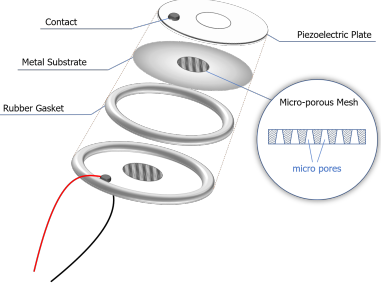
\includegraphics[width=0.55\columnwidth]{./img/piezo-transducer.png}
  \caption{Micro-porous mesh piezoelectric transducer for ultrasonic diffusion --- withdrawn from~\cite{wen2019development}}%
\label{fig:piezo-transducer}
\end{figure}

This micro-porous piezoelectric transducer is driven by an \gls{ac} signal at a
frequency of around 113 kHz and converts electric energy into kinetic energy due
to inverse-piezoelectricity~\cite{wen2019development}. The metal substrate
vibrates along with the vibration of the ring-shaped piezoelectric plate, and
the mesh in the center of the metal substrate smashes the liquid beneath the
transducer. Some liquid flows through those micro-pores and is emitted in
micro-droplet form, due to the momentary vacuum created.

The rationale behind the micro-porous piezoelectric is due to its
versatility regarding voltage supply, small size, easy control, low power
consumption and variety of fluids that it can diffuse.
A list of micro-porous piezoelectric film properties are listed below~\cite{wen2019development}:
\begin{enum-c}
\item Diameter: 13.8 mm.
\item Low driving voltage: 3--12 V.
\item High conversion efficiency, spray volume.
\item Exit aperture is very small 4 µm.
\item Frequency: 113 kHz ± 5 kHz.
\item Capacitance: 2700 PF ± 15\%.
\item Power: 1.5--2.0 W.
\item Spray volume 30 ml/h.
\item Can atomize essential oils, perfume, water based perfumes or even mixture
  of the mentioned materials.
\item life of more than 3000 hours.
\end{enum-c}

Abid et al.~\cite{abid2015novel} proposed a novel olfactory displays' scent
dispersing module based on this type of transducer
(Fig.~\ref{fig:novel-olfactory-scent-elem}). It contains a refillable fragrance
reservoir, a cotton core and the housing for the micro-porous piezoelectric
film. The fragrance ascends to the cotton core via capillary effect,
impregnating it. When the micro-porous electric film is stimulated the fragrance
in the cotton core is diffused through the aforementioned effect.
%
\begin{figure}[htb!]
\centering
    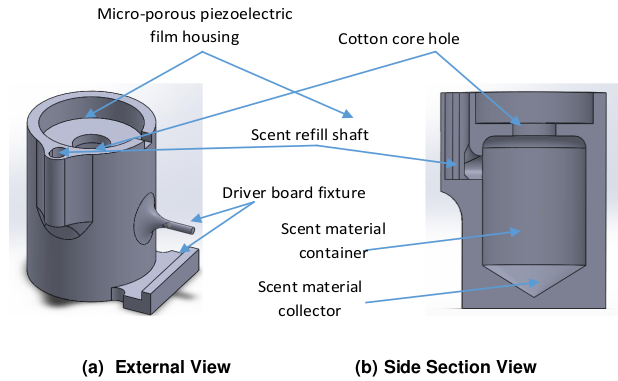
\includegraphics[width=0.65\columnwidth]{./img/novel-olfactory-scent-elem.png}
  \caption{Micro-porous mesh piezoelectric-based scent dispense module --- withdrawn from~\cite{abid2015novel}}%
\label{fig:novel-olfactory-scent-elem}
\end{figure}

\subsubsection{Driving circuit}
\label{sec:driving-circuit}
There are several commercially available \glspl{pcb} to drive micro-porous
piezoelectric transducers. Fig.~\ref{fig:pcb-diffusion} illustrates a commercial
\gls{pcb} to drive piezoelectric transducer of 113 kHz resonance frequency.
%
\begin{figure}[htb!]
\centering
    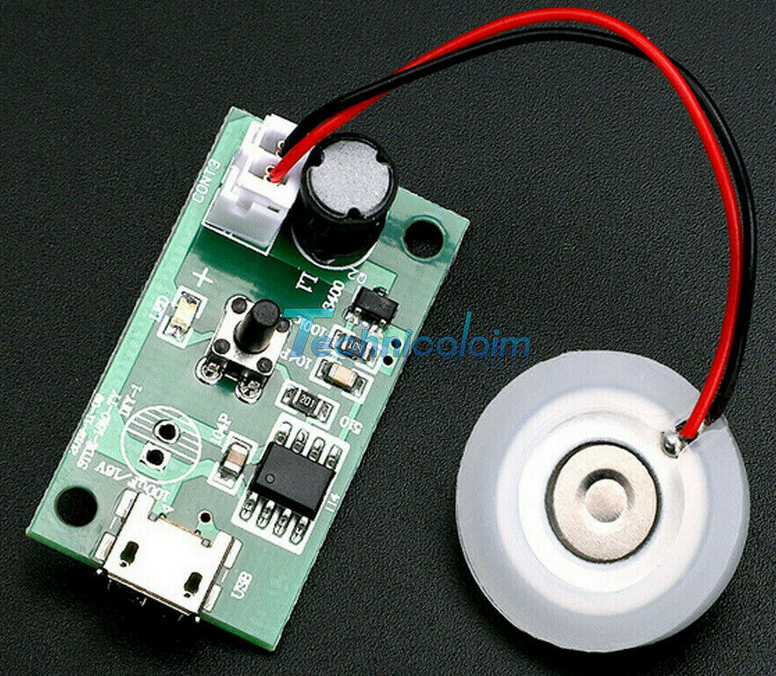
\includegraphics[width=0.4\columnwidth]{./img/pcb-diffusion.png}
  \caption{Commercial \gls{pcb} for driving micro-porous mesh piezoelectric transducers~\cite{ebayPiezo}}%
\label{fig:pcb-diffusion}
\end{figure}

As aforementioned, piezoelectric transducers for diffusion require an \gls{ac}
signal at the resonance frequency. Fig.~\ref{fig:pcb-reverse-eng} illustrates a
possible driving circuit for these transducers. A 555-timer \gls{ic} is used in
astable mode to generate a square wave at the resonance frequency that drives a
gate of power \gls{mosfet}. This \gls{mosfet} which feeds an resonant circuit to
generate an \gls{ac} signal which stimulates the piezoelectric transducer,
producing mechanical oscillations at the resonance frequency. This application
requires a fast-switching power \gls{mosfet}, like the IRLZ44N, as the
piezoelectric transducer consumes up to 300 mA of current. 
%
\begin{figure}[htb!]
\centering
    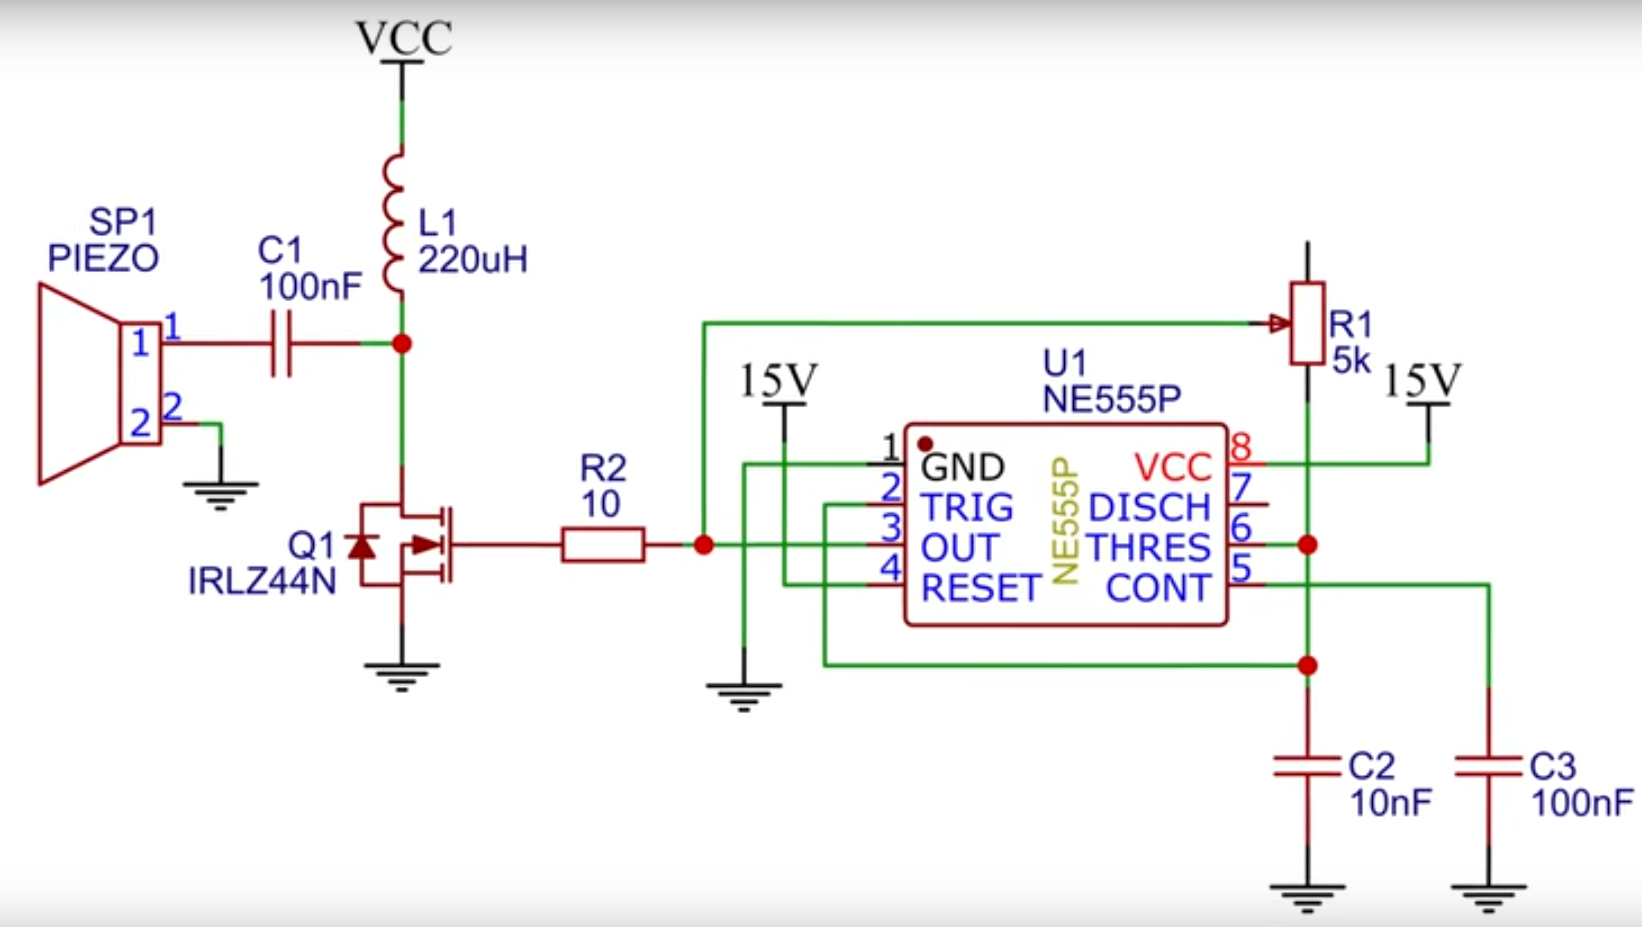
\includegraphics[width=0.6\columnwidth]{./img/pcb-reverse-eng.png}
  \caption{Schematic of a driving circuit for micro-porous mesh piezoelectric transducers~\cite{piezoSchematic}}%
\label{fig:pcb-reverse-eng}
\end{figure}



%%% Local Variables:
%%% mode: latex
%%% TeX-master: "../../../dissertation"
%%% End:
